\documentclass[a4peper, 12pt, titlepage, finall]{extreport}

%различные пакеты

\usepackage[T1, T2A]{fontenc}
\usepackage[russian]{babel}
\usepackage{tikz}
\usepackage{geometry}
\usepackage{indentfirst}
\usepackage{fontspec}
\usepackage{graphicx}
\graphicspath{{./images/}}

\usetikzlibrary{positioning, arrows}

\geometry{a4paper, left = 15mm, top = 10mm, bottom = 20mm, right = 15mm}

\setmainfont{Times New Roman}
\setmonofont{Courier New}
\setcounter{secnumdepth}{0}
%\setcounter{tocdepth}{3}

\begin{document}

    \begin{titlepage}
        \begin{center}
            {\small \sc Московский государственный университет имени М.~В.~Ломоносова\\
            Факультет вычислительной математики и кибирнетики\\
            Кафедра автоматизации систем вычислительных комплексов\\}
            \vfill
            {\large \sc Обзор}\\~\\

            {\large \bf Анализ и исследование алгоритмов поиска в архитектуре сетевого процессора без выделенного ассоциативного устройства.}\\~\\

        \end{center}
        
        \begin{flushright}
            \vfill
            {Никифоров Никита Игоревич, 321 группа}
        \end{flushright}

        \begin{center}
            \vfill
            {\small Москва\\2019}
        \end{center}
    \end{titlepage}

    \tableofcontents
    \listoffigures
    \newpage
    \section{Аннтотация}
        В настоящее время активно развиваются ПКС сети, в них используются многофункциональные программируемые коммутаторы. 
        Перед нашей кафедрой стоит задача создания такого коммутатора, основным элементом которого является сетевое процессорное устройство, далее СПУ. 
        СПУ — устройство на котором решаются задачи классификации и маршрутизации пакетов, то есть от
        СПУ требуется отделить тело пакета от заголовка, обработать заголовок, и присоединить новый заголовок обратно к телу пакета. 
        Одна из важнейших особенностей СПУ — их программируемость, а именно возможность загрузить на СПУ любую программу обработки пакетов.  
        Это необходимо, чтобы один и тот же коммутатор мог выполнять разные сетевые задачи, без этого при необходимости решить новую задачу пришлось бы создавать новый коммутатор.
        Также программируемость позволяет сторонним разработчикам сетевых приложений быстро разворачивать свой продукт на ПКС сетях. 
        При создании высокопроизводительных программируемых СПУ возникает множество проблем, таких как: 
        \begin{enumerate}
            \item Долгий процесс разработки СПУ, цикл может длиться до 5 лет
            \item {\ttfamily TODO Дописать проблемы создания СПУ}
            \item Сложность создания базовых алгоритмов и структур данных для работы СПУ

        \end{enumerate}
        В данной работе я рассмотрю проблему разработки алгоритма и структуры данных для классификации пакетов. 
        В рассматриваемой архитектуре СПУ отсутствует выделенное ассоциативное устройство. 

    \section{Введение}
        В рассматриваемой архитектуре СПУ используется конвейерная архитектура, конвейер состоит из десяти вычислительных блоков, 
        далее ядра конвейера, они идентичны между собой. TODO Ещё одной особенностью архитектуры СПУ является то, что все данные хранятся в коде программы. 
        Созданием и модификацией структуры данных занимается отдельное вычислительное устройство ЦПУ.
        Целью данного обзора является выбор наиболее подходящих алгоритмов и структур данных для реализации их в СПУ. 
        Для выбора алгоритмов для реализации было необходимо разработать критерии оценки алгоритмов. 
        Они обоснованы особенностями архитектуры и необходимостью оценки производительности алгоритмов.
    \section{Цели и задачи}
        Целью моей работы было исследовать и разработать структуру данных и алгоритм для поиска в
        рамках архитектуры СПУ без выделенного ассоциативного устройства.
        Для достяжения цели необходимо было выполнить следующие задачи:
        \begin{enumerate}
            \item Ознакомиться с основными понятиями ПКС с акцентом на плоскость передачи данных, языком программирования сетевых устройств P4, архитектурой отечественного сетевого процессора.
            \item Провести обзор алгоритмов LPM поиска с целью выбора для применения в рассматриваемой архитектуре процессора.
            \item Разработать критерии сравнения алгоритмов поиска с акцентом на применимость в рассматриваемой архитектуре.
            \item Реализовать выбранные алгоритмы поиска в эмуляторе сетевого процессора.
            \item Провести экспериментальное исследование реализованных алгоритмов.
        \end{enumerate}
    
    \newpage

    \section{Постановка задачи}
        Моей задачей было исследование, сравнение и реализация алгоритмов и структур данных для поиска в таблицах классификации пакетов. 
        В силу особенностей архитектуры СПУ, а именно отсутствие адресуемой  памяти, 
        которая требуется для  алгоритмов поиска будут рассматриваться только древовидные структуры данных. 
        Под памятью занимаемой структурой данных понимается  {\ttfamily   N * 128 = memmory} , где {\ttfamily N} - количество 
        инструкций в конкретной реализации рассматриваемой структуры данных, 128 - бит на одну инструкцию.

    \section{Критерии обзора}
        В обзоре были использованы следующие критерии:
        \begin{enumerate}
            \item Асимтотическая сложность поиска - позволяет оценить использование ресурсов СПУ, для поиска в структуре данных.
            \item Универсальность структуры данных - используемая структура данных должна поддерживать поиск любых данных не превосходящих по размеру 128 бит и представимых в двоичном виде.
            \item Дополнительные данные не обходимые для построения древовидной структуры.
            \item Необходимость использования адресуемой памяти - некоторым рассматриваемым структурам данных требуется адресуемая память для их реализации, соответствующей их асимптотической сложности.
            \item Количество вершин, которое мы проходим для поиска в худшем случае.
            \item Возможность оптимизации алгоритма поиска с помощью инструкций микроархитектуры ядерконвейера СПУ.
            \item Необходимость изменения микроархитектуры ядер конвейера СПУ.
            \item Оценка памяти занимаемой структурой данных - рассматривается структура данных для 10000 вождений префиксов IPv4.
            \item Сложность добавления и удаления элементов из рассматриваемой структуры данных.
        \end{enumerate}

        Сравнение структур данных будет провоодиться по критериям 1, 2, 4, 5, 8.

    
    \newpage

    \section{Структуры данных}
        \subsection{Binary one bit tree}
            Наиболее распространенная структура данных для LPM. Строится дерево по заданным префиксам, 
            так что каждому биту префикса соответствует своя вершина в дереве. 
            Поиск осуществляется спуском в глубину по битам элемента, для которого выполняется поиск. 
            Поиск заканчивается тогда, когда достигнута пустая вершина, результатом поиска считается последний встретившийся префикс. 
            На Рис. 1 изображено данное дерево для набора префиксов.

            \begin{figure}[h]      
                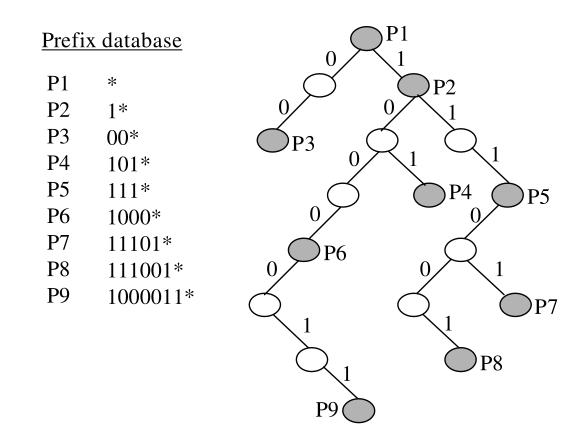
\includegraphics[width=\textwidth]{one_bit_tree.png}
                \caption{Однобитное дерево}
                \label{fig:mesh1}
            \end{figure}

            \underline{Асимптотическая сложность поиска для этой структуры данных} соответствует {\ttfamily $\log_2{W*N}$},\\
            где {\ttfamily W} - максимальная длина префикса, а {\ttfamily N} -- количество префиксов в структуре данных.\\
            \underline{Универсальность структуры данных} - рассматриваемое дерево может быть использовано для любых данных представимых в битовом виде.\\
            \underline{Дополнительные данные для построения структуры данных} не требуются.\\
            \underline{Количество вершин которое необходимо посетить для поиска} не превосходит 128.\\
            \underline{Оптимизацию агоритма поиска} проводить не требуется.\\
            \underline{Изменение микроархитектуры ядер конвейера СПУ} не требуется для реализации данного алгоритма.\\
            \underline{Оценка памяти занимаемой структурой данных} - рассматриваемая структура данных занимает не более чем 15000Кбайт.\\
            \underline{Добавление и удаление элементов из рассматриваемой структуры данных} имеет логарифмическую сложность, и не требует перестройки всей структуры данных.\\

        \subsection{Path compressed trie (PATRICIA trie)}
            Эта структура данных -- пришедшая со временем оптимизация Binary one bit tree. Оно сжимается, 
            то есть все вершины у которых только один лист сокращаются, и в следующую вершину заносятся данные о 
            количестве пропущенных вершин, таким образом данное дерево не имеет вершин с одним листом. Благодаря этому данное дерево
            занимает гораздо меньше памяти, потому что нет проходных вершин, но уменьшает количество затраченных инструкций на поиск лишь 
            для некоторых префиксов и в худшем случае оно аналогично Binary one bit tree.

            \begin{figure}[h]
                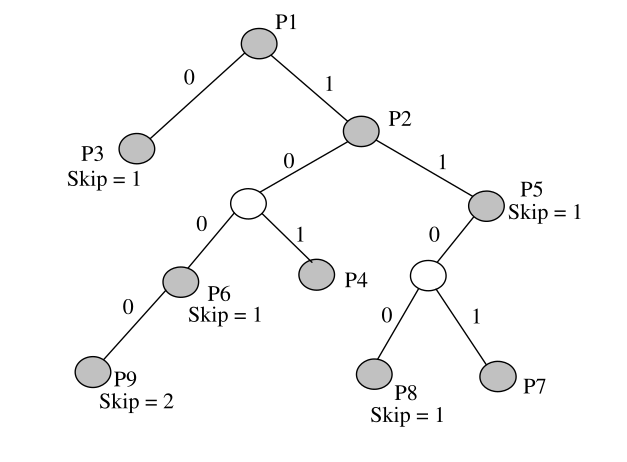
\includegraphics[width=\textwidth]{patricia_trie.png}
                \caption{PATRICIA Trie}
                \label{fig:mesh2}
            \end{figure}

            \underline{Асимптотическая сложность поиска для этой структуры данных} соответствует {\ttfamily $\log_2{N*W}$},\\
            где {\ttfamily W} - максимальная длина префикса, а {\ttfamily N} -- количество префиксов в структуре данных.\\
            \underline{Универсальность структуры данных} - рассматриваемое дерево может быть использовано для любых данных представимых в битовом виде.\\
            \underline{Дополнительные данные для построения структуры данных} не требуются.\\
            \underline{Количество вершин которое необходимо посетить для поиска} не превосходит 128.\\
            \underline{Оптимизацию агоритма поиска} проводить не требуется.\\
            \underline{Изменение микроархитектуры ядер конвейера СПУ} не требуется для реализации данного алгоритма.\\
            \underline{Оценка памяти занимаемой структурой данных} - рассматриваемая структура данных занимает не более чем 8000Кбайт.\\
            \underline{Добавление и удаление элементов из рассматриваемой структуры данных} имеет логарифмическую сложность, и не требует перестройки всей структуры данных.\\

        \subsection{Level Compressed Trie}
            Данное дерево -- следующая оптимизация Path Compressed Trie. Используется другая конццепция деревьев, когда в каждой вершине
            может быть максимум не два листа, а {\ttfamily $2^h$}, где {\ttfamily h} -- это максимальная глубина поддерева данной вершины.
            При использование рассматриваемой структуры данных в рамках архитектуры ЦПУ, количество операций для поиска ограничевается глубиной дерева,
            которая равна {\ttfamily $\frac{W}{K}$}, где {\ttfamily W} -- длина максимального префикса, а {\ttfamily K} -- количество уровней в нашем дереве.
            В рамках архитектуры СПУ, невозможно реализовать адресуемый доступ к памяти, поэтому будет рассматриваться реализация данного дерева,
            в которой используется линейный поиск в каждой вершине по уровням.

            \begin{figure}[h]
                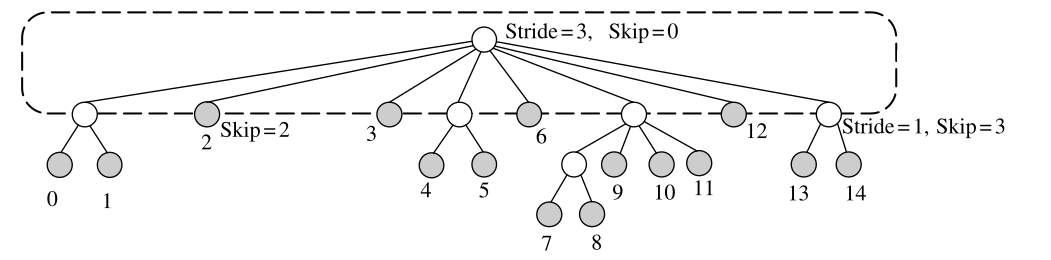
\includegraphics[width=\textwidth]{level_compressed_trie.png}
                \caption{Level Compressed Trie}
                \label{fig:mesh3}
            \end{figure}

            \underline{Асимптотическая сложность поиска для этой структуры данных} соответствует {\ttfamily $\frac{W}{K}*N$},\\
            где {\ttfamily K} - количество префиксов в рассматриваемой структуре данных, а {\ttfamily W} - максимальная длина префикса.
            и {\ttfamily N} -- количество листьев в вершине.\\
            \underline{Универсальность структуры данных} - рассматриваемое дерево может быть использовано для любых данных представимых в битовом виде.\\
            \underline{Дополнительные данные для построения структуры данных} не требуются.\\
            \underline{Количество вершин которое необходимо посетить для поиска} не превосходит 30.\\
            \underline{Оптимизацию агоритма поиска} нужна, для организации бастрого доступа к листьям внутри одной вершины.\\
            \underline{Изменение микроархитектуры ядер конвейера СПУ} требуется аппаратная реализации быстрого перехода внутри одной вершины.\\
            \underline{Оценка памяти занимаемой структурой данных} - рассматриваемая структура данных занимает не более чем 18000Кбайт.\\
            \underline{Добавление и удаление элементов из рассматриваемой структуры данных} имеет логарифмическую сложность, и не требует перестройки всей структуры данных.\\


        \newpage

        \subsection{Binary Search on Prefix Lengths}
            Алгоритм основан на построении специальных таблиц для префиксов определённой длины, если у нас максимальная длина префикса {\ttfamily W}, 
            то строятся Таблицы {\ttfamily $h_{1}...h_{w}$}. В каждой из них хранятся префиксы длины соответствующие номеру этой Таблицы. Предполагается, 
            что в каждой такой таблице реализована своя хеш-функция, которая быстро позволяет найти вхождение префикса в данную таблицу, 
            таким образом мы можем сделать бинарный поиск по длине префиксов. В рамках рассматриваемой архитектуры СПУ, реализация таких таблиц возможна только
            с использованием древовидных структур данных.

            \begin{figure}[h]
                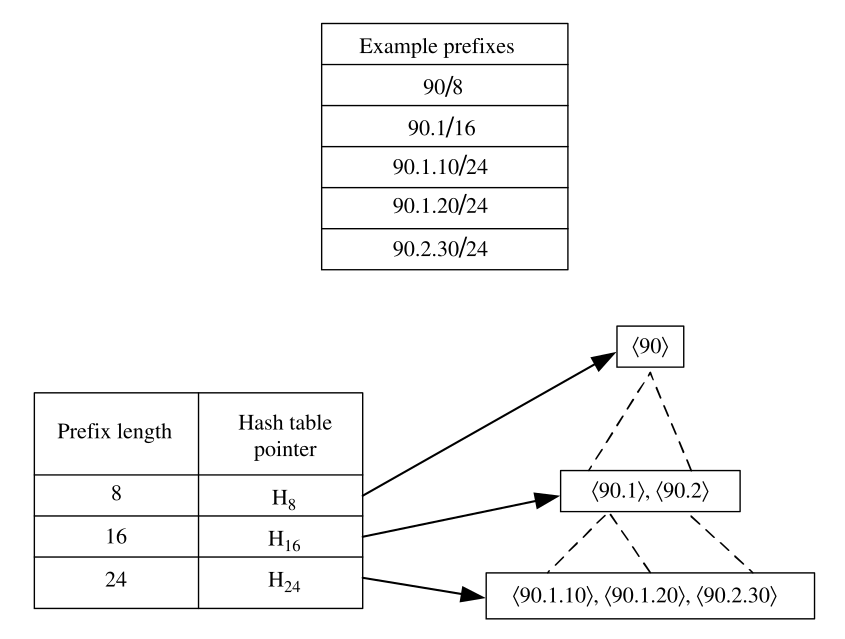
\includegraphics[width=\textwidth]{binary_search.png}
                \caption{Binary Search of Prefix Lengths}
                \label{fig:mesh4}
            \end{figure}

            \underline{Асимптотическая сложность поиска для этой структуры данных} соответствует {\ttfamily $K*\log_2{N}$},\\
            где {\ttfamily K} - количество префиксов в рассматриваемой структуре данных, а {\ttfamily W} - максимальная длина префикса.
            и {\ttfamily N} -- количество префиксов в таблице.\\
            \underline{Универсальность структуры данных} - рассматриваемая структура данных может быть использовано только для поиска префиксов.\\
            \underline{Дополнительные данные для построения структуры данных} не требуются.\\
            \underline{Количество вершин которое необходимо посетить для поиска} не превосходит 128.\\
            \underline{Оптимизацию агоритма поиска} необходима для реализации поиска внутри таблицы.\\
            \underline{Изменение микроархитектуры ядер конвейера СПУ} требуется аппаратная реализация хеш-функций.\\
            \underline{Оценка памяти занимаемой структурой данных} - рассматриваемая структура данных занимает не более чем {\ttfamily TODO: рассчитать} Кбайт.\\
            \underline{Добавление и удаление элементов из рассматриваемой структуры данных} требует перестройки всей структуры данных.\\


        \subsection{Scalar Prefix Search (AVL Tree)}
            Данный флгоритм позволяет представлять префиксы как скалярные величины, что позволяет для них использовать больший набор структур данных. 
            В качестве примера рассмотрим AVL дерево, основной особенностью которого является правило его построения: у каждой вершины разность 
            глубины левого и правого поддерева не превосходит 1, что даёт ассимптотическую сложность поиска {\ttfamily $1+\log{N}$}, 
            где {\ttfamily N} -- количество префиксов в нашей структуре данных. Из этого следует, что время поиска не зависит от длины искомых данных,
            а значит с помощью данной структуры данных очень эффективно выполнять поиск префиксов IPv6.
            \\
            \\
            {\ttfamily TODO найти картинку}
            \begin{figure}[h]
                \caption{AVL Tree}
                \label{fig:mesh5}
            \end{figure}
            \\
            \\
            \underline{Асимптотическая сложность поиска для этой структуры данных} соответствует {\ttfamily $1 + \log_2{N}$},
            где {\ttfamily N} -- количество префиксов в таблице.\\
            \underline{Универсальность структуры данных} - рассматриваемое дерево может быть использовано для любых данных представимых в битовом виде.\\
            \underline{Дополнительные данные для построения структуры данных} не требуются.\\
            \underline{Количество вершин которое необходимо посетить для поиска} не превосходит 20.\\
            \underline{Оптимизацию агоритма поиска} проводить не требуется.\\
            \underline{Изменение микроархитектуры ядер конвейера СПУ} не требуется.\\
            \underline{Оценка памяти занимаемой структурой данных} - рассматриваемая структура данных занимает не более чем {\ttfamily TODO: рассчитать} Кбайт.\\
            \underline{Добавление и удаление элементов из рассматриваемой структуры данных} имеет логарифмическую сложность, и не требует перестройки всей структуры данных.\\

        \newpage

    \section{Сравнение структур данных}
        Для сравнения структур данных построим таблицу сравнения по критериям: ассимптотическая сложность, универсальность структуры данных,
        количество вершин, которое необходимо поситить для поиска и оценка памяти занимаемой структурой данных.
        \\
        \\
        \begin{tabular}{lcccc}
            \bf Название структуры & \bf Сложность & \bf Универсальность & \bf Количество вершин & \bf Память \\
            Binary one bit tree & $\log_2{W*N}$ & да & 128 & 15000 \\
            Path Compressed trie & $\log_2{W*N}$ & да & 128 & 8000 \\
            Level Compressed trie & $\frac{W}{K}*N$ & да & 32 & 18000 \\
            Binary Serarch on prefix length & $K*\log_2{N}$ & нет & 128 & {\ttfamily TODO} \\
            AVL Tree & $1 + \log{N}$ & да & 20 & {\ttfamily TODO} \\
        \end{tabular}

    \section {Выводы}
        {\ttfamily TODO: написать выводы, сделаю это позже, потому что пока не могу полностью оценить рассматриваемые структуры данных.}
\end{document} 
